\documentclass[11pt,twocolumn]{article}
\usepackage{amsmath}
\usepackage[margin=1in]{geometry}
\usepackage{graphicx}
\usepackage{import}
\usepackage{subfig}

\title{Vision-Based Autonomous Ground Vehicle Navigation}
\date{March 31, 2011}
\author{
	Michael Koval \\
	mkoval@eden.rutgers.edu \\
	Electrical and Computer Engineering
}

\begin{document}
\maketitle

\section{Introduction}
\label{sec:intro}
% 1. Overall description of IGVC
The Intelligent Ground Vehicle Competition (IGVC) is an international
collegiate robotics competition that tasks teams of undergraduate students to
design, build, and program a fully autonomous mobile ground vehicle.
Specifically, a successful vehicle vehicle must be capable of navigating
through a narrow obstacle course, visiting waypoints in an open field, and
travelling between global positioning system (GPS) scattered throughout a
field, and responding to Joint Architecture for Unmanned Systems (JAUS)
messages ~\cite{igvc11}.

% 2. Importance of Perception
In each of these tasks, the team knows only the destination waypoint with no
knowledge of the course's actual topology. Sucessfully remaining within the
course boundaries while avoiding obstacles requires that the robot be able to
both build and localize itself within a map of drivable regions. This is
further complicated by the use of a narrow painted lines to delimit the course
boundaries and the large variety of road obstacles to block the path, including
cones, barriers, potholes, and switchbacks ~\cite{igvc11}.

% 3. Overview
Finding these obstacles has historically been accomplished using a scanning
laser range finder (LIDAR) and computer vision to build a local map of the
robot's environment ~\cite{princeton08} ~\cite{delaware08}. Before discussing
specific algorithms, Section ~\ref{sec:robot} provides a brief introduction to
the hardware and software used on Rutgers University's IGVC entry. The body of
the paper is split into two major sections: the use of stereo vision for
obstacle detection (Section ~\ref{sec:stereo}) and monocular image processing
to track the course boundary lines (Section ~\ref{sec:line}). Finally, Section
~\ref{sec:future} addresses potiential planned improvements to the vision
system and Section ~\ref{sec:econ} expands the topic to the recent interest
in robotic disaster recovery systems.

\section{Rutgers Navigator}
\label{sec:robot}
% 1. Brief discussion of mechanical design
Designed specifically for rugged outdoor use and modularity, the Rutgers
Navigator is constructed entirely out of 80/20 extrusion and custom-machined
alumninum stock. This provides a strong, light\footnote{Approximately 100 lb
empty and 150 lb fully loaded.} frame that is much
easier to modify than a welded steel frame. This frame is supported by three
wheels: two powered front wheels mounted on a wish bone suspension and
free-spinning rear castor selected to reduce friction when turning via
differential drive.

\begin{figure}
	\center
	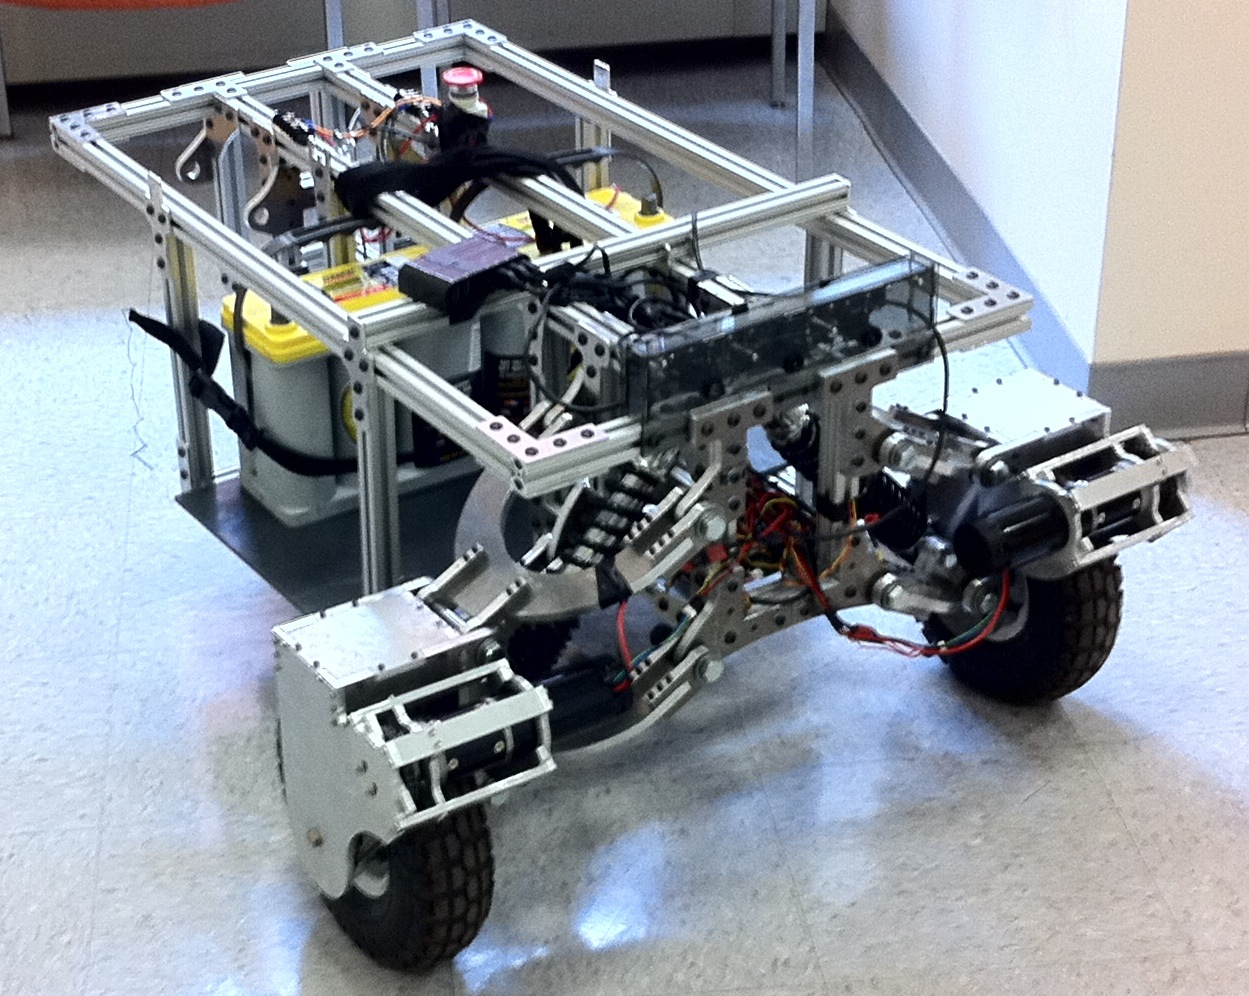
\includegraphics[width=\linewidth]{include/robot-photo}
	\caption{Rutgers Navigator robot}
	\label{fig:robot-photo}
\end{figure}

% 2. Sensing capabilities
\subsection{Sensing Capabilities}
\label{sec:robot-sensors}
Each of the drive motors that attached to the front wheels are equipped with
internal hall-effect quadrature encoders to measure wheel speed and a current
sensor to monitor power consumption. The local odometry information captured by
the wheel encoders is combined with the data produced by a nine-axis intertial
measurement unit (IMU) that contains and accelerometer, gyroscope, and magnetic
compass to estimate the robot's motion. Conversely, the robot's absolute
position is found using a high-end Nortel differential global positioning
system (DGPS) that is accurate within 50 cm under normal operation and 10 cm
using OmniStar's correction service ~\cite{omnistar}.

As was discussed in Section ~\ref{sec:intro}, precise knowledge of the robot's
position is not sufficient to successfully complete the challenges. Instead,
knowledge of the robot's local environment is collected using a Hokuyo LIDAR
and a custom trinoculur stereo vision system that is discussed in detail in
Section ~\ref{sec:stereo}. Combining the planar point cloud measured by the
LIDAR with the full three-dimensional information produced by stereo vision
results in an aggregate point cloud with both the field of view and granularity
necessary to successfully avoid obstacles.

\subsection{Software Architecture}
\label{sec:robot-software}
Interaction between the robot's individual software components will be
connected the Robot Operating System (ROS), a framework developed by Willow
Garage to promote code reuse in robotics. Besides providing a common interface
to libraries such as OpenCV and PCL, ROS encourages the separation of software
into a graph of loosely-coupled \textit{nodes} that communicate over TCP/IP
sockets ~\cite{ros}. Because each node \textit{subscribes} to its inputs and
\textit{publishes} its outputs with no global knowledge of the system, it is
possible to reuse nodes without any knowledge of their internal structure.

\begin{figure}
	\centering
	\includegraphics[width=\linewidth]{include/robot-software-vision}
	\caption{Computer vision software subsystem.}
	\label{fig:robot-vision}
\end{figure}

Using the concept of a node to model the complete computer vision subsystem
produces the graph shown in Figure ~\ref{fig:robot-vision} (see Appendix
~\ref{sec:robot-graph} for the complete graph of interactions). Within this
graph, there are three distinct processing piplines: stereo vision, monocular
lane tracking, and monocular object recognition. As its name suggests, the
\textit{stereo vision} pipeline (Section ~\ref{sec:stereo} uses triplets of
synchronized images to generate a three-dimensional point cloud used to
identify obstacles. The monocular \textit{line tracking} (Section
~\ref{sec:line}) pipeline identifies white boundary lines in each input image
and tracks position relative to the robot over time. Finally, the
\textit{object recognition} pipeline identifies purely visual targets and
obstacles such as ``simulated potholes''\footnote{Ellipses placed on the grass
to simulate real potholes.} and flags.

% 4. Gazebo Simulation
% FIGURE: Photo of simulated environment
% TODO: maybe...

\section{Stereo Reconstruction}
\label{sec:stereo}
% 1. Selection of the PS3 Eye camera
Stereo vision on a mobile robot is a non-trivial problem that has traditionally
required costly hardware that support high frame rates and hardware
synchornization, such as the Bumblebee stereo vision camera. Thankfully, the
inexpensive Playstation Eye camera uses the OmniVision OV7720 capable of frame
rates up to 125 Hz and can be easily modified to support hardware
synchronization. Mounted in a custom polycarbinate case (Figure
~\ref{fig:sec:stereo-camera}), three of these cameras are used for stereo
reconstruction.

% 2. Hardware and software camera synchronization
% FIGURE: Justification for synchronization
% FIGURE: Synchronized and desynchronized osilloscope output
% FIGURE: Synchronized and desynchronized images of a clock
\subsection{Synchronization}
\label{sec:stereo-sync}
Even if the cameras used for stereo reconstruction are attached to the same
computer and set to the same frame rate, there is no guarantee that frames will
be captured simultaeously from both cameras. If the cameras are in motion (such
as being attached to a moving robot) this delay changes the effective baseline
of the stereo system and invalidates the camera calibration\footnote{Assuming a
framerate of 30 Hz and a velocity of 10 mph, the effective baseline could change
by up to 7 cm.} that was used when stationary. As the change in the system's
baseline is a function of both the robot's velocity and the extent of the
desynchronization, it is impossible to compensate for its effects.

\begin{figure*}
	\centering
	\subfloat[Unsynchronized \texttt{VSYNC}]{
		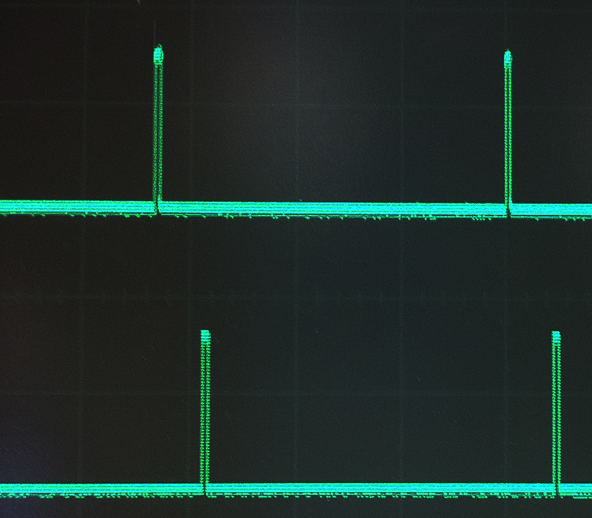
\includegraphics[width=0.24\textwidth]{include/unsync-scope}
		\label{fig:stereo-sync-hard1}
	}
	\subfloat[Synchronized \texttt{VSYNC}]{
		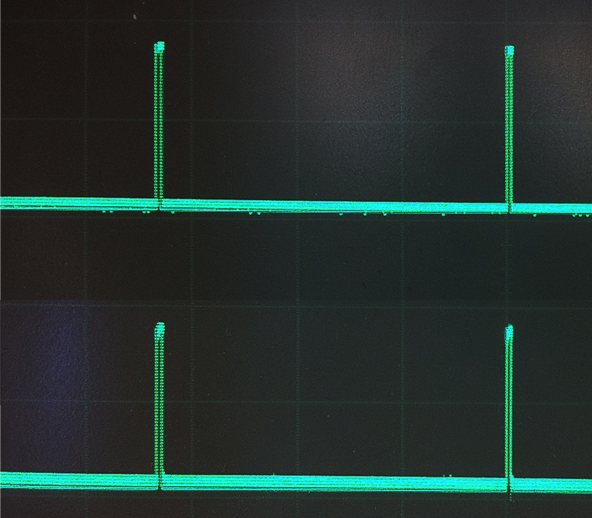
\includegraphics[width=0.24\textwidth]{include/sync-scope}
		\label{fig:stereo-sync-hard2}
	}
	\subfloat[Unsynchronized Frames]{
		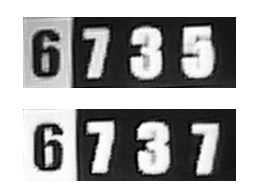
\includegraphics[width=0.24\textwidth]{include/unsync-img}
		\label{fig:stereo-sync-soft1}
	}
	\subfloat[Synchronized Frames]{
		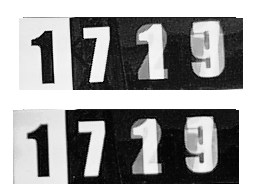
\includegraphics[width=0.24\textwidth]{include/sync-img}
		\label{fig:stereo-sync-soft2}
	}
	\caption{
		Verification of hardware and software camera synchronization for two
		Playstation Eye cameras. Note how only the synchronized cameras share a
		common \texttt{VSYNC} clock and capture identical readings of a
		millisecond resolution timer.
	}
	\label{fig:stereo-sync}
\end{figure*}

Hardware synchronization was achieved by  shorting the frame clock
(\texttt{VSYNC}) of the ``master'' camera to the frame trigger inputs
(\texttt{FSIN}) of the ``slave'' cameras. For electrical safety, each of the
cameras' USB grounds were shorted to force a common ground. This
synchronization guarantees that the cameras capture images simultaneously, but
does not guarantee that the images will be synchronized after the USB transfers
to the computers. Making direct use of the Video4Linux kernel module, software
synchronization was achived by fuzzy-matching of the the USB transfer
timestamps\footnote{\texttt{https://github.com/mkoval/stereo\_webcam}}.
Synchronization was verified in hardware by probing each camera's
\texttt{VSYNC} pin with an osilloscope (Figures ~\ref{fig:stereo-sync-hard1}
and ~\ref{fig:stereo-sync-hard2}) and and in software by recording images of a
millisecond-resolution timer (Figures ~\ref{fig:stereo-sync-soft1} and
~\ref{fig:stereo-sync-soft2}).

% 3. Baseline multiplexing using three cameras
% FIGURE: Effect of baseline on dead zone and maximum range.
% FIGURE: Graph of distance vs. disparity for both baselines.
% FIGURE: Graph of distance vs. error for both baselines.
\subsection{Baseline Multiplexing}
\label{sec:stereo-mux}
While unknown changes in the system's baseline is disasterous, having control
over the stereo camera's baseline can be extremely beneficial. Selecting the
best baseline is a balance of two opposing, but equally important, factors:
dead-zone and range. Decreasing the baseline shrinks the both the size of the
deadzone and the maximum range at which distances can be distinguished. This
maximum range exists because disparity is measured in pixels: there is no
discernable difference between any disparity less than one pixel. Multiplexing
between a 10 cm baseline (the \textit{narrow stereo}) and a 20 cm baseline (the
\textit{wide stereo}) combines the benefits of both baselines.

\begin{figure*}
	\centering
	\subfloat[Multiplexed Point Cloud]{
		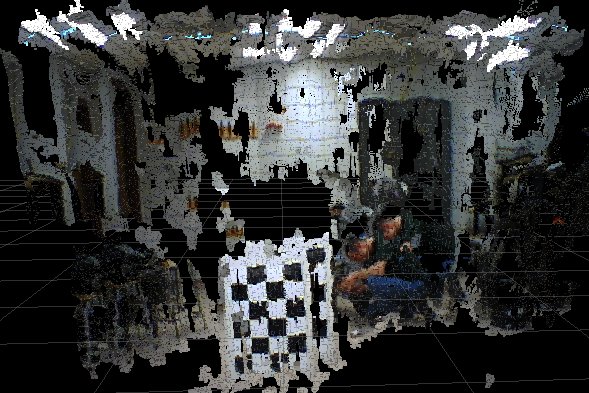
\includegraphics[width=0.5\linewidth]{include/stereo-both}
	}
	\subfloat[Reconstruction Error]{
		\subimport{include/}{stereo-dist}
	}
	\caption{
		Reconstructed point cloud using stereo multiplexing. Differences in the
		camera's rectification and reconstruction accuracy cause a small
		rotation in the reconstructed point cloud.
	}
\end{figure*}

For a stereo camera, the relationship between distance and disparity can be
shown to be
\begin{equation*}
	x = \frac{bf}{n\sigma}
\end{equation*}
where $b$ is the baseline, $f$ is the camera's focal distance, and $\sigma$ is
the size of a pixel on the image sensor. By substituting the intrinsics
parameters of the Playstation Eye camera\footnote{$f = 3.15$ mm, $\sigma = 6$
$\mu$m} and setting $n = 1$ pixel, the maximum range of both baselines can be
evaluated. As can be seen in Figure ~\ref{fig:stereo-dist-disparity}, the 10 cm
and 20 cm baselines have theoretical maximum ranges of 5 m and 10 m
respectively. With the width of the course fixed at approximately 6 m, a
maximum range of 10 m is more than sufficient for navigation purposes.

% 5. Point correspondances: SSD BM on the CPU or SAD BM on the GPU?
% TODO: FIGURE: Sample reconstructed point cloud
% TODO: Discussion of parameter selection
% TODO: Statistical outlier detection using PCL.
\subsection{Reconstruction Algorithm}
\label{sec:stereo-correspond}
Due to the use of ROS as the basis for the Navigator's software architecture
(Section ~\ref{sec:robot}), the actual stereo reconstruction is done using the
standard \texttt{stereo\_image\_proc} ROS node. This node implements real-time
calibrated stereo by rectifying the images, applying a texture-enhancing
filter, and using a sum-of-squared difference (SSD) block-matching algorithm to
point correspondences. This disparity map is then converted into a
three-dimensional point cloud in the cameras' coordinate frame using the
calibration parameters.

\subsection{Error Analysis}
% TODO: How!?

\section{Lane Tracking}
\label{sec:line}
For both the navigation and GPS challenges, the drivable region of the course
is delimited by a three inch wide line painted on the grass or asphalt.
Robustly identifying and tracking these lane boundary lines is a non-trivial
problem that has been the primary cause of disqualifications in previous years
of competitions. For example, 28 out of 29 competitors were disqualified before
time elapsed in the 2010 Intelligent Ground Vehicle Competition.

The algorithm discussed below is a modified version of the algorithm used by
MIT's entry into the DARPA Grand Challenge. In this algorithm, a color image
of the course undergoes a color spae transformation to emphasize white regions
of the image (Section ~\ref{sec:line-color}). The grayscale output of the color
space transformation is then filtered using a matched pulse-width filter
(Section ~\ref{sec:line-filter}) and compressed with non-maximal supression
(Section ~\ref{sec:line-max}). These local maxima are then transformed into
the world coordinate frame using the robot's estimated state and are tracked
over time through model fitting (Section ~\ref{sec:line-model}).

\begin{figure*}
	\subfloat[Original Image]{
		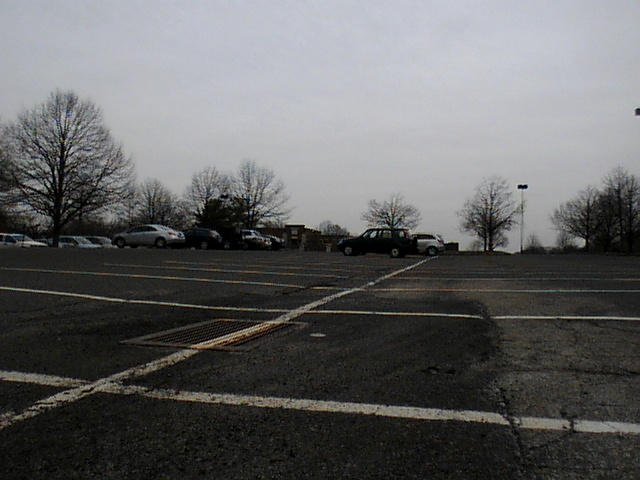
\includegraphics[width=0.5\linewidth]{include/line-orig}
	}
	\subfloat[Color Space Transformation]{
		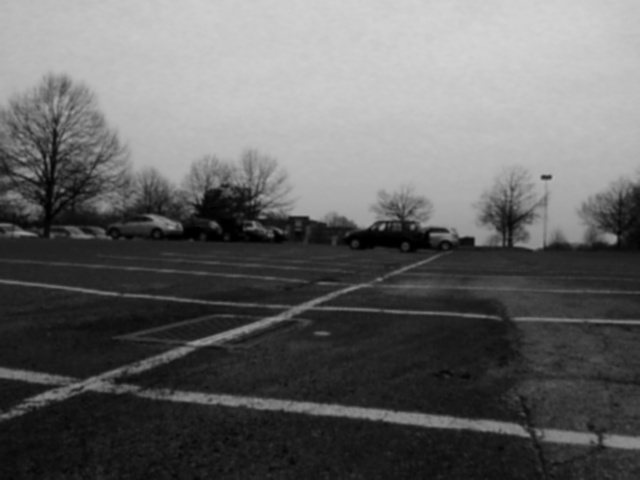
\includegraphics[width=0.5\linewidth]{include/line-pre}
	}
	\\
	\subfloat[Matched Pulse-Width Filter]{
		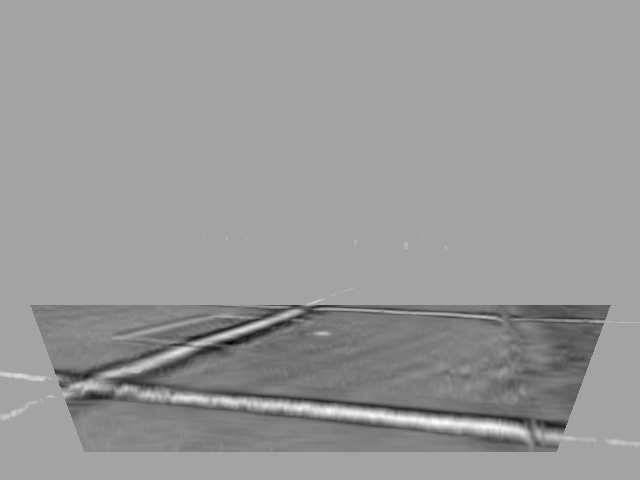
\includegraphics[width=0.5\linewidth]{include/line-filter}
	}
	\subfloat[Non-Maximal Suppression]{
		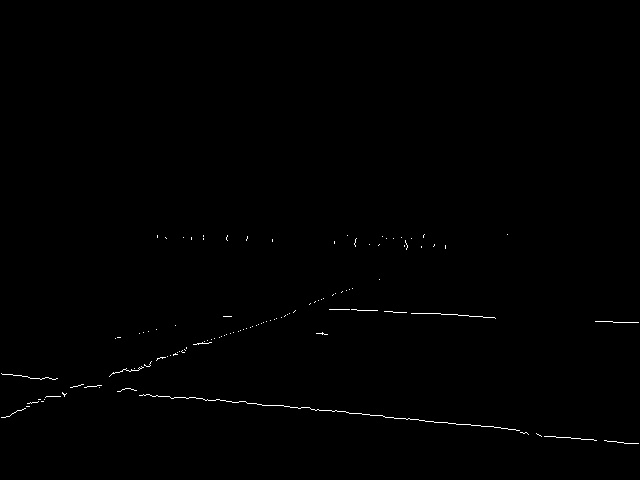
\includegraphics[width=0.5\linewidth]{include/line-max}
	}
	\caption{Intermediate stages of the line detection algorithm.}
	\label{fig:lane-all}
\end{figure*}

% 1. Color space transformation
\subsection{Color Space Transformation}
% TODO


% 2. Creating and using a matched pulse-width filter (!)
\subsection{Matched Pulse-Width Filter}
Because the lines on the course are known to be uniformly three inches wide, an
obvious approach for isolating them from other objects is to use a digital
\textit{pulse-width filter} that is of the same width. Unfortunately, the
effects of perspective projection mean that the apparent width of lines in the
image depend upon their distance from the camera. To obtain useful output, such
a filter must be properly \textit{matched} to expected width of the line at
each point in the image.

Calculating this width requires knowledge of the three-dimensional point
corresponding to each pixel in the image. Assuming that the ground plane is
known and is parameterized by point $P$ and normal $n$, the three-dimensional
point $P$ that corresponds to pixel $p$ satisifes both
\begin{align*}
	(P - P_0) \cdot n     &= 0 \\
	\lambda M^{-1}_{int} p - P &= 0,
\end{align*}
where $M_{int}$ is the camera's intrinsic matrix and $\lambda$ is an arbitrary
constant.

Solving for $\lambda$ results in a closed-form expression containing
only known parameters. Substituting this value into the equation of the
line yields an intersection point of
\begin{equation*}
 	P = \left(\frac{n \cdot P_0}{n \cdot M^{-1}_{int} p}\right) M^{-1}_{int} p.
	\label{eq:line-point}
\end{equation*}
Using the new-found knowledge of point $P$, the pixel-width of the pulse-width
filter matched to pixel $p$ can easily be computed as
\begin{equation*}
	w = ||M_{int} P - M_{int} (P + W)||_2
\end{equation*}
where $W$ is a vector in direction $\langle 1, 0, 0 \rangle$ for a horizontal
line or $\langle 0, 0, 1 \rangle$ for a vertical line and $||\cdot||_2$ denotes
the Euclidean norm. Note that this is not equivalent to $||W||_2$ because of
the division implicit in the use of homogeneous coordinates.

Once the expected width of the line at a given pixel is determined, seperate
horizontal and vertical pulse-width filters are created. Each of these filters
consists of a positive \textit{pulse} of width $w$ surrounded on both sides by
negative \textit{supports} of width $\frac{w}{2}$, normalized to have a zero
sum. When implemented, a rectified input image was used to guarantee that depth
does not vary within a row of pixels. This allows one filter to be pre-computed
per row, dramatically improving the algorithm's practical performance.

% FIGURE: Output of the pulse-width filter in each direction

% 3. Non-maximal Supression
\subsection{Non-Maximal Suppresion}
\label{sec:line-nonmax}
The matched pulse-width filter is extremely effective at isolating the line in
the image, but does not produce a clean enough output to be directly used for
model-fitting. In particular, the nature of digital filters guarantees that
there will be weak, spurious responses near true positives.

Inspired by Canny edge detection, non-maximal supression is an effective and
computationally efficient way of reducing such a response to a single point.
Considering the rows of the horizontally filtered image and the columns of the
vertically filtered image, a pixel is considered a maximum if and only if it
has a higher filter response than both of its neighbors. The maxima are then
thresholded to discard those that do not exhibit a sufficiently strong filter
response. This threshold was tuned to favor false positives and was set to
approximately 15\% of the filter's maximum response.

% TODO: Output of non-maximal suppression

% 4. Model Fitting
\subsection{Model Fitting}
\label{sec:line-model}
% TODO: Actually implement this...
% FIGURE: Output of model fitting.

% 5. Error Analysis
% TODO: Number of false positives versus deviations in ground plane
% TODO: Number of false positives versus deviations in line width
% TODO: Number of false positives versus 

\section{Conclusion}
\label{sec:conclusion}
% ???

\section{Future Work}
\label{sec:future}
% 1. Obstacle detection using the stereo point cloud
% 2. Use stereo depth information to mask line false positives
% 3. Stereo and/or IMU-based ground plane detection
% 4. Use normal vectors to fit bicubic splines
% 5. Basic object recognition for flags, potholes, and road obstacles
% 6. Ground plane detection with stereo/kinect/imu

\section{Economics}
\label{sec:econ}
% TODO

\section{Acknowledgements}
% TODO: Make this phrasing less awkward.
This project would not have been possible without the support of Dr. Predrag
Spasojevic as our faculty advisor or the help of the members of Rutgers IEEE
Student Branch. I am particulary grateful for Adam Stambler's excellent
leadership, Peter Vasilnak's mechanical design, and the faculty support of Dr.
Kristin Dana, Joe Lippencott, Steve Orbine, John Scafidi, and Dr. Stuart
Shalat. I would also like to thank our sponors: Rutgers Engineering Governing
Council, Knotts Corporation, 80/20 Inc., Optima Batteries, Github, IEEE Region
1, Novatel, and Omnistar.

\appendix
\section{Software Architecture}
\label{sec:robot-graph}
\begin{figure*}
	\centering
	\includegraphics[width=\linewidth]{include/robot-software-all}
	\label{fig:robot-software-all}
\end{figure*}

\section{Source Code}
Digital access to all code is available online upon request via a private
Github respository.

% 1. stereo_webcam
% 2. stereo_mux
% 3. line_detection
% 4. line_tracker
% 5. camera_calibration modification (???)

\end{document}
